% Equal scalar shifts attain both spectral perturbation bounds.
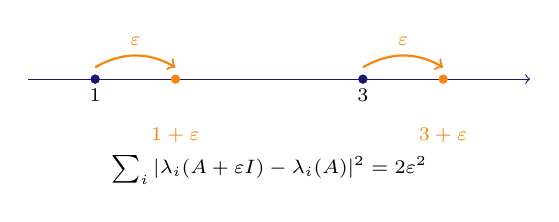
\begin{tikzpicture}[x=1.7cm,y=1cm,every node/.style={font=\scriptsize}]
\draw[->,MidnightBlue] (0.5,0)--(4.25,0);
\foreach \a/\b in {1/1.6,3/3.6}{
\fill[MidnightBlue] (\a,0) circle (1.7pt);
\fill[BurntOrange] (\b,0) circle (1.7pt);
\draw[->,BurntOrange,thick] (\a,0.15) to[bend left=30] node[above] {$\varepsilon$} (\b,0.15);
}
\node[below] at (1,0) {$1$};\node[below] at (3,0) {$3$};
\node[BurntOrange,below=14pt] at (1.6,0) {$1+\varepsilon$};
\node[BurntOrange,below=14pt] at (3.6,0) {$3+\varepsilon$};
\node at (2.3,-1.15) {$\sum_i|\lambda_i(A+\varepsilon I)-\lambda_i(A)|^2=2\varepsilon^2$};
\end{tikzpicture}
